\chapter{Experiments}\label{ch:experiments}
All experiments described in this chapter are executed in a test environment at NIKHEF. The test environment is displayed in image \ref{fig:testenv}.

\begin{figure}
  \includegraphics[scale=0.45]{images/testenv.pdf}
  \caption{Used environment for experiments.}
  \label{fig:testenv}
\end{figure}

Three identical servers (A, B and C)  are used to perform the tests. Table \ref{tab:testmachines} contains the specifics of the three servers. 
These servers are all connected to a Juniper QFX10k2 (device S). This switch has 32 40Gb/s QFSP ports. 
Some of these ports are configured as a 100Gb/s interface. 
During the experiments 2 extra machines are introduced into the network. Both containing 100Gb/s Mellanox cards.
Table \ref{tab:ppc-intel} contains the information about the extra machines.   

\todo[inline]{make tables for machines}

Device A is always the receiving end of the test. Depending on the tests the source can be machine B, C or B and C.
For possible +40Gb/s tests, one of the 100Gb/s machines (D or E) can be used.

Machine M is a Simple Network Management Protocol (SNMP) server. This SNMP server query's the machines every second for status. 
As seen in the image of the test environment \ref{fig:testenv}. SNMP is active on a different interface of the devices.  

\section{RFC}\label{sub:rfc}
Multiple RFC's are written that provide guidelines for throughput testing.
Terms from RFC1242 \cite{rfc1242} will be used during this research and techniques from RFC2544 \cite{rfc2544} will be considered to be used during this research.
RFC6349 \cite{rfc6349} describes a framework for TCP throughput testing. The framework is using iPerf to perform the tests.
RFC6815 \cite{rfc6815} describes why RFC2544 should not be followed in production environments. Unfortunately it doesn't offer any extra's. 

A quick list with guidelines from these RFC's is as follows:

\begin{itemize}
\item{Throughput tests should have a minimum runtime of 30 seconds}
\item{The environment cannot be a production environment}
\item{DUT's will be overloaded}
\end{itemize} 

\section{Basic tools}
Some of the basic tools are used to see the possibilities of the tooling. 
\subsection{iPerf3}
IPerf3 is a client server based tool that allows packet generation. Machine A is setup as a server running on default TCP port 5201, machine B is setup as a client connecting to the server. 
First sending 64 bytes of traffic in each packet. The maximum amount of packets was not reached until 6 threads where used to generate traffic. All of the cores where running at 100\%. 40Gb/s was reached when 16 threads ran with packets of 1500bytes. When using packets of 9000 bytes, only 2 threads needed to run at the same time to reach 40Gb/s. The fact that iPerf3 is capable of sending traffic over one single TCP session per thread makes it less useful for this project.

\subsection{Hping}
Hping is used to send spoofed traffic to a server. 100 syn requests per second produced a maximum of 13Gb/s of traffic towards a server when packets of 9000bytes are being transferred. Although it has some nice features and probably has the capacity to bring down certain web servers, the bandwidth usage is to less for this project. It is very useful for testing open ports in firewalls.  

\subsection{Bonesi}
The maximum output that was produced with BoNeSi was 300Mb/s and 500Kpps. This is not sufficient for this project and therefore BoNeSi will not be used during further testing. A source IP list can be created, so it can be used to simulate traffic from different locations inside the network to check if firewall rules are setup correctly and traffic is allowed to flow from different sources inside the network. For this scenario, high bandwidth is not necessary and BoNeSi is a solid solution. Next to the bandwidth, 500Kpps with sessions is enough to overload a small firewall.  

\section{DPDK}
The Data Plane Development Kit (DPDK) offers the possibility of bypassing the kernel, reserving CPU, memory and interfaces to do one task. The hardware is capable of talking directly to each other without interrupts. In order to reach 40Gb/s of data at leyer 4 and op to layer 7 makes is the main goal for this research. Lets see what is has to offer. 

\subsection{PKTGEN}
For this experiment, like all others, destination is server A, source is server B. Both machines are identical as seen in table \ref{tab:testmachines}. Pktgen is not a client server based application. System A is idle, B will generate traffic. Performance testing between UDP and TCP did not show significant differences between the two protocols. To get some hardware specifics Pktgen was set to send 64 byte packet at the maximum possible rate. This ended up in 42Mpps where the expected amount of packets is 56Mpps unidirectional. The Intel card seems to be the bottleneck here. The DPDK website offers a guide to setup the system in order to get the maximum performance out of the Intel XL710 40Gb/s card. Flashing a new firmware version into the card was a first step. After following the guide the result remained the same. According to conclusion drawn out of a report from Chelsio \cite{chelsio} the PCI express bus is capable of transferring 70Mpps bidirectional. Unidirectional it can reach a maximum of 42Mpps. Scaling up the packet size from 64 bytes to 1024 bytes resulted in a sweet spot of a bandwidth usage of 39.8Gb/s and a total of 11Mpps. Figures \ref{fig:pktgenlink} and \ref{fig:pktgenpps} display the amount of bandwidth transferred and the amount of pps transferred during the tests using 400 byte packets

\begin{figure}
  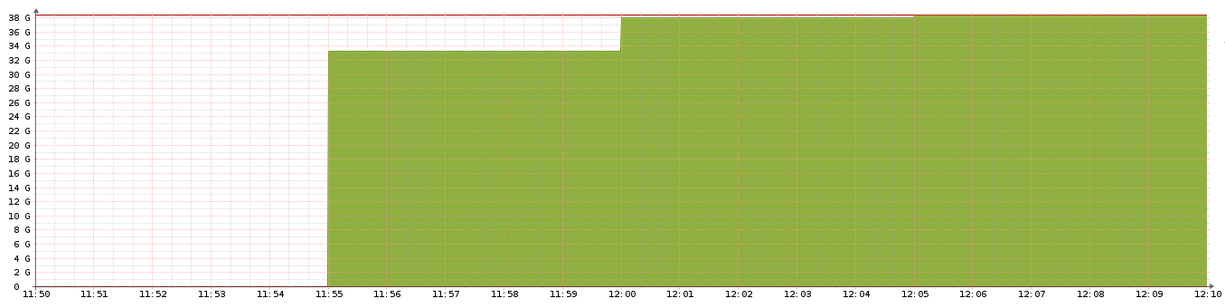
\includegraphics[scale=0.35]{images/pktgen_link_usage.png}
  \caption{Pktgen link usage}
  \label{fig:pktgenlink}
\end{figure}

\begin{figure}
  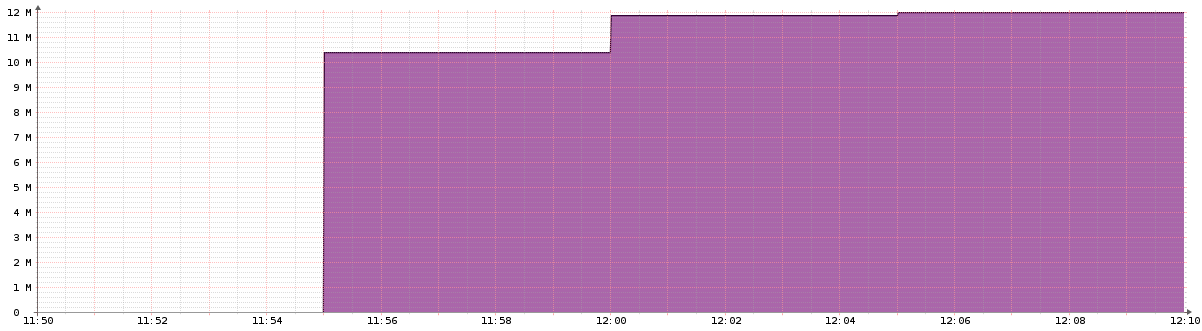
\includegraphics[scale=0.35]{images/pktgen_pps.png}
  \caption{Pktgen packets per second}
  \label{fig:pktgenpps}
\end{figure}


\subsection{WARP17}
A WARP client needs a server to respond to syn packets, otherwise sessions are not opened up and there will be no traffic on the line. 
WARP has to be tested against a WARP server or against an application server. 
So server A became a WARP server and machine B is generating responses. RAW TCP communication is chosen for a first test. Sending a request of 64 bytes and responding with 64 bytes did not generate the maximum amount of pps. WARP should not be used to create a large amount of pps. 
To execute a benchmark for warp, server B was connected to the network over 2 interfaces. 
The results of this back2back tests for raw tcp traffic is visible in figures \ref{fig:rawtcplink} and \ref{fig:rawtcpsession}. 
WARP is also capable of testing HTTP session setup. The results of this benchmark is visible in figures \ref{fig:httplink} and \ref{fig:httpsession}.
These figures show us the packet sizes from the request and response along with the amount of session or the link usage.

\begin{figure}
  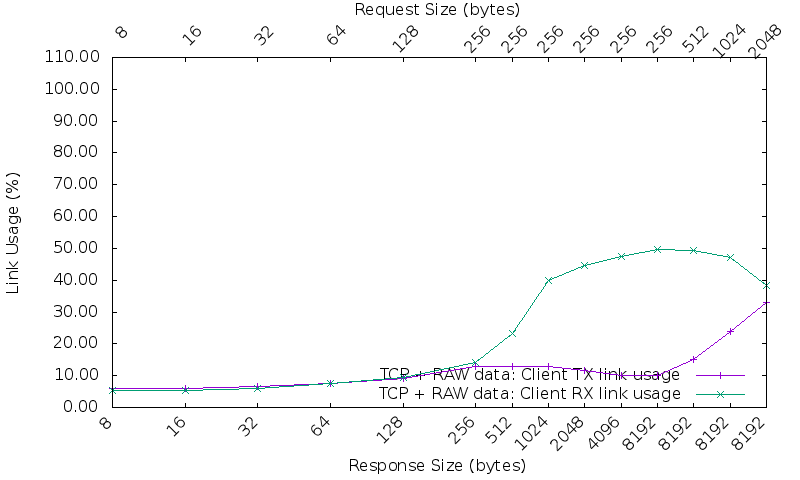
\includegraphics[scale=0.6]{images/raw_link_usage.png}
  \caption{Link usage for raw tcp}
  \label{fig:rawtcplink}
\end{figure}

\begin{figure}
  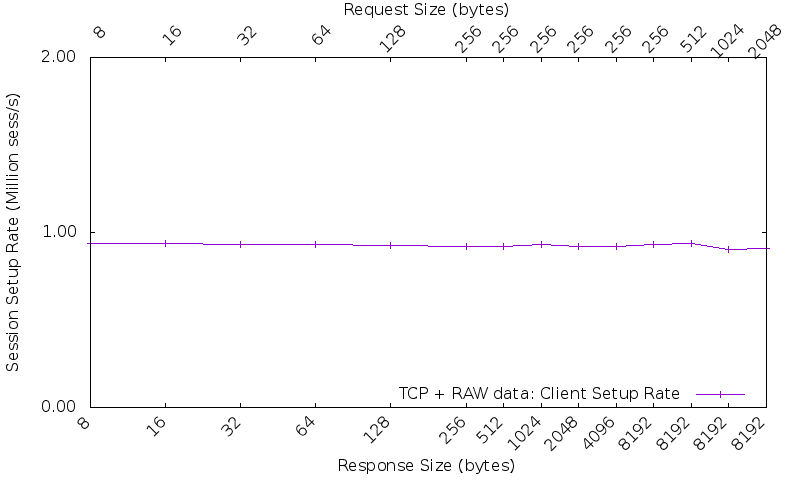
\includegraphics[scale=0.6]{images/raw_setup.png}
  \caption{Amount of session per second for raw tcp.}
  \label{fig:rawtcpsession}
\end{figure}

\begin{figure}
  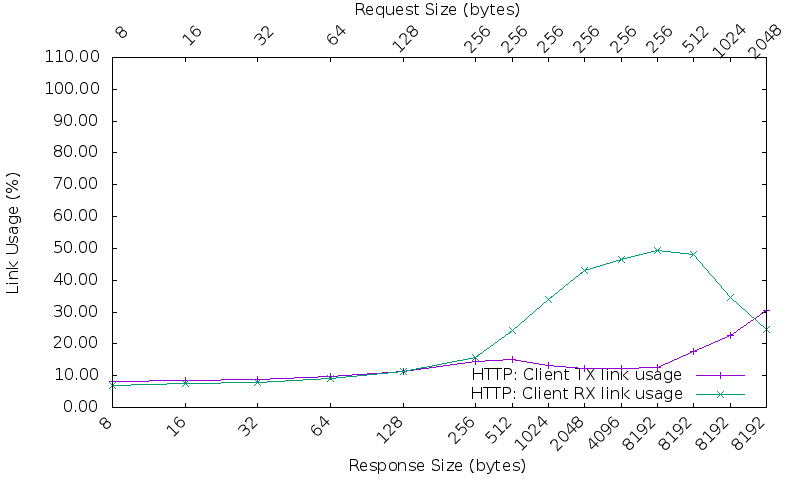
\includegraphics[scale=0.6]{images/http_link_usage.png}
  \caption{link usage for http}
  \label{fig:httplink}
\end{figure}

\begin{figure}
  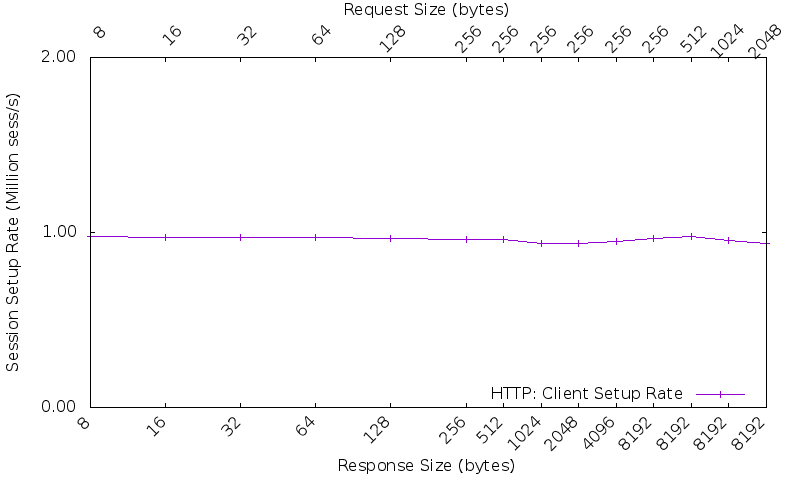
\includegraphics[scale=0.6]{images/http_setup.png}
  \caption{Amount of sessions per second for http}
  \label{fig:httpsession}
\end{figure}


\subsection{Moongen}

\todo[inline]{insert images of client, server and network load}



